\documentclass[dvipsnames]{beamer}
\usepackage[utf8]{inputenc}
\usepackage[spanish]{babel}
\usepackage{subfigure, wrapfig}
\usepackage{multirow}
\usepackage{graphicx}
\usepackage{hyperref}
\usepackage{tikzsymbols}

\date{} %not show date

%beamer's options
\usetheme{Montpellier}
\author{Gustavo Rivas Gervilla}
\title{Spark \& IoT}

\setbeamertemplate{section in toc shaded}[default][50]
%beamer's colors
\setbeamercolor{section in toc}{fg=orange}
\setbeamercolor{section in toc shaded}{fg=orange}
\setbeamercolor{structure}{fg=brown}
\setbeamercolor{title}{fg=brown}
\setbeamercolor{titlelike}{fg=brown}

%defined colors
\definecolor{deepBlue}{RGB}{10, 9, 68}
\definecolor{deepYellow}{RGB}{219, 219, 8}
\definecolor{deepRed}{RGB}{130, 20, 6}
\definecolor{orangeRed}{RGB}{211, 50, 10}
\definecolor{redBrown}{RGB}{99, 7, 7}

%hyperref setup
\hypersetup{
     colorlinks   = true,
     linkcolor = brown,
     urlcolor = redBrown
}

\begin{document}
	\begin{frame}[plain]
		\titlepage
	\end{frame}
		
	\begin{frame}
		\frametitle{Contenido}
		\tableofcontents
	\end{frame}
	
	\AtBeginSection[]{
		\begin{frame}
			\frametitle{Contenido}
			\tableofcontents[currentsection]
		\end{frame}
	}
	
	\section{Introducción}
	
        \begin{frame}
          \begin{itemize}
          \item Muchos dispositivos de diversa naturaleza.
          \item Intercambio y envío de información \textbf{continuo}.
          \item \textcolor{deepRed}{Gran cantidad} de datos de diversa naturaleza $\Rightarrow$ \textcolor{SkyBlue}{\textbf{CC}}. 
          \end{itemize}
        \end{frame}

        \begin{frame}
          \begin{itemize}
          \item En 2020 habrá un cuarto de billón de vehículos conectados [Gartner] $\Rightarrow$ \textbf{muchos datos}.
          \item Analizando estos datos podemos analizar tráfico de una zona o detectar si un conductor no está en condiciones de conducir.
          \item Se propone \textcolor{orange}{\textbf{Spark}} para analizar todos estos datos.
          \end{itemize}
        \end{frame}

        \begin{frame}
          \begin{itemize}
          \item Proyecto académico.
          \item Analizar y procesar datos de vehículos $\Rightarrow$ Panel de monitorización
          \item En su \href{https://github.com/baghelamit/iot-traffic-monitor}{\textcolor{deepBlue}{GitHub}} tenéis todo el código disponible \Winkey.
          \end{itemize}
        \end{frame}

        \begin{frame}
          \begin{center}
          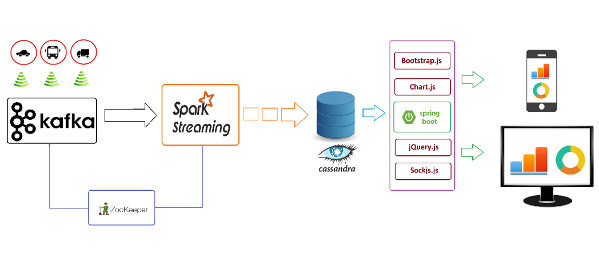
\includegraphics[scale=0.3]{img/arquitectura.jpg}  
          \end{center}          
        \end{frame}

        \section{Kafka: producir}
	
	\begin{frame}
          \begin{figure}[H]
            \centering
            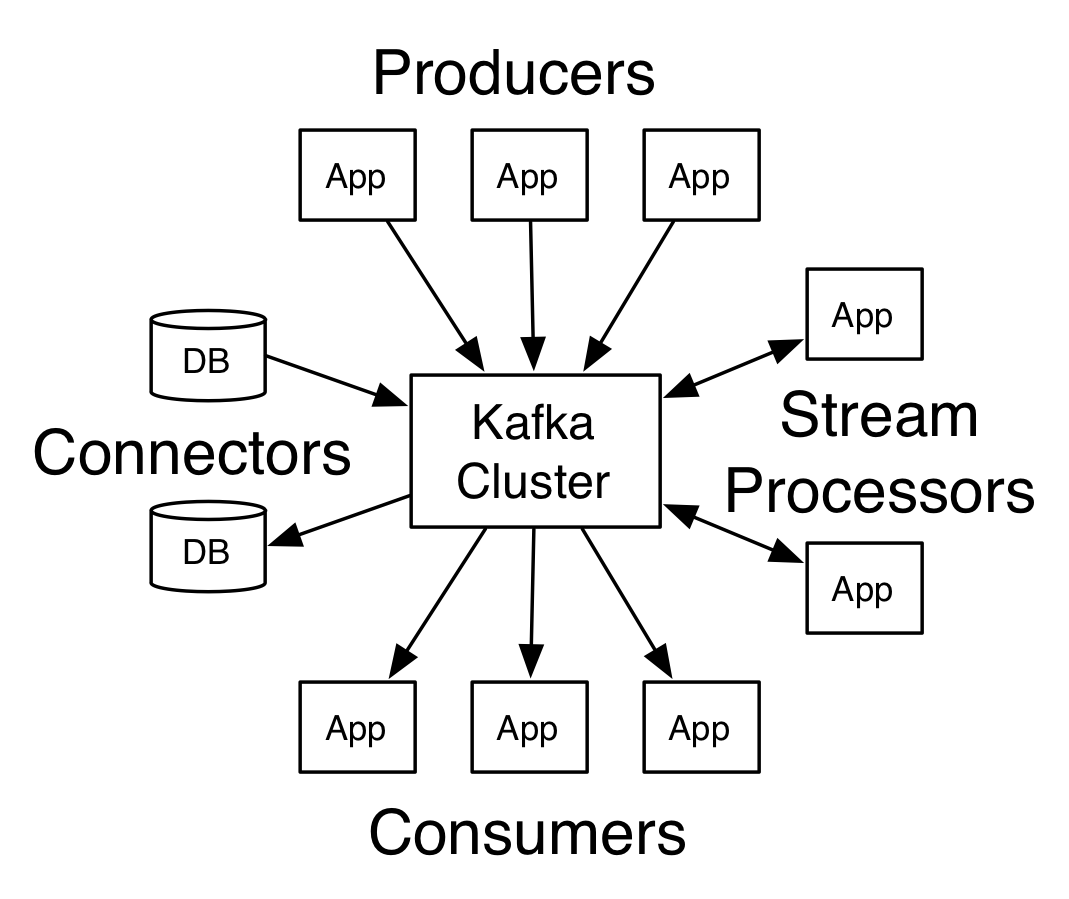
\includegraphics[scale=0.7]{img/kafka-apis.png}
          \end{figure}
          \begin{itemize}
          \item Mensaje $:=$ \{clave, valor, instante\} $\in$ stream $\in$ topics $\in$ log particionado $\Rightarrow$ \textcolor{deepRed}{tolerancia a fallos}.
          \item Lo mejor del sistema de colas (división de tareas) y lo mejor del modelo publicar-subscribir (\textit{broadcasting}).
          \item Conservan el orden de los mensajes.
          \end{itemize}
	\end{frame}
	
	\section{Spark Streaming: procesar}
	
	\begin{frame}
          ¿Qué es Spark?
          \begin{itemize}
          \item Código abierto.
          \item Sistema de propósito general para el procesamiento de Big Data en un sistema cluster.
          \item APIs en: \textcolor{deepBlue}{Python}, \textcolor{deepRed}{Scala} y \textcolor{orangeRed}{Java}.
          \end{itemize}
	\end{frame}	
	
	\begin{frame}
          ¿Y Spark Streaming?
          \begin{itemize}
          \item Extensión para aplicaciones de procesamiento de datos en tiempo real.
          \item Puede leer datos de HDFS, \textbf{Kafka}, Twitter y ZeroMQ. Además de los que definamos nosotros.
          \item Tolerancia a fallos sin esfuerzo por parte del programador \Smiley.

            \begin{figure}[H]
              \centering
              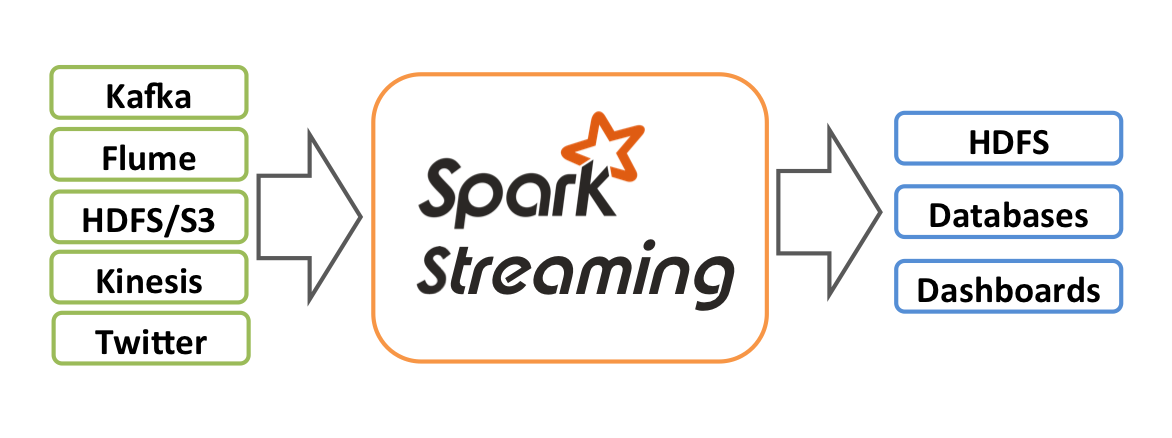
\includegraphics[scale=0.4]{img/streaming-arch.png}
            \end{figure}

            
          \item El procesamiento de los datos tan complejo como se necesite.
          \end{itemize}          
	\end{frame}

        \begin{frame}
          \begin{figure}[H]
            \centering
            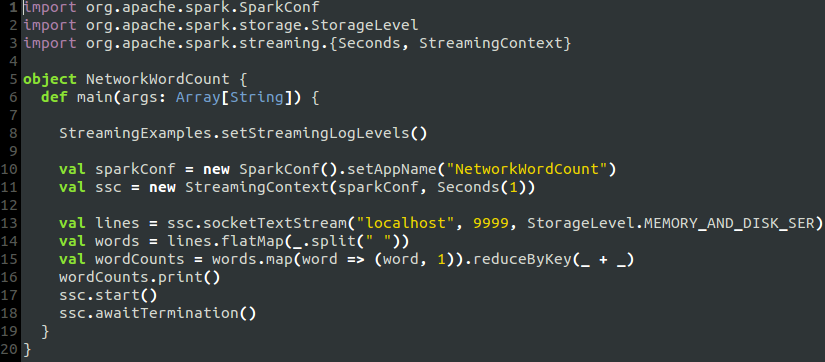
\includegraphics[scale=0.4]{img/script.png}
          \end{figure}
        \end{frame}

        \begin{frame}
          \begin{itemize}
          \item La interfaz de Python es algo limitada. 
          \item Se especifica un ``flujo'' que luego se ejecuta.
          \item \texttt{map, reduce, join, reduceByKey...}
          \item Permite operar por ventanas.
          \item Podemos tener \textcolor{deepRed}{replicación} (\texttt{StorageLevel}).
          \item $\frac{\text{Tolerancia a fallos}}{\text{RDD + recuperación del Driver + replicación}}$
          \end{itemize}
        \end{frame}
        
        \section{Cassandra: almacenar}

        \begin{frame}
          \begin{itemize}
          \item Tolerancia a fallos \& Durabilidad.
          \item Rendimiento.
          \item Disponibilidad.
          \item Elasticidad.
          \item Descentralizada.
          \item Escalabilidad. \textcolor{deepRed}{Escalabilidad de escritura} (varios \textit{masters}).
          \end{itemize}

          \begin{figure}[H]
            \centering
            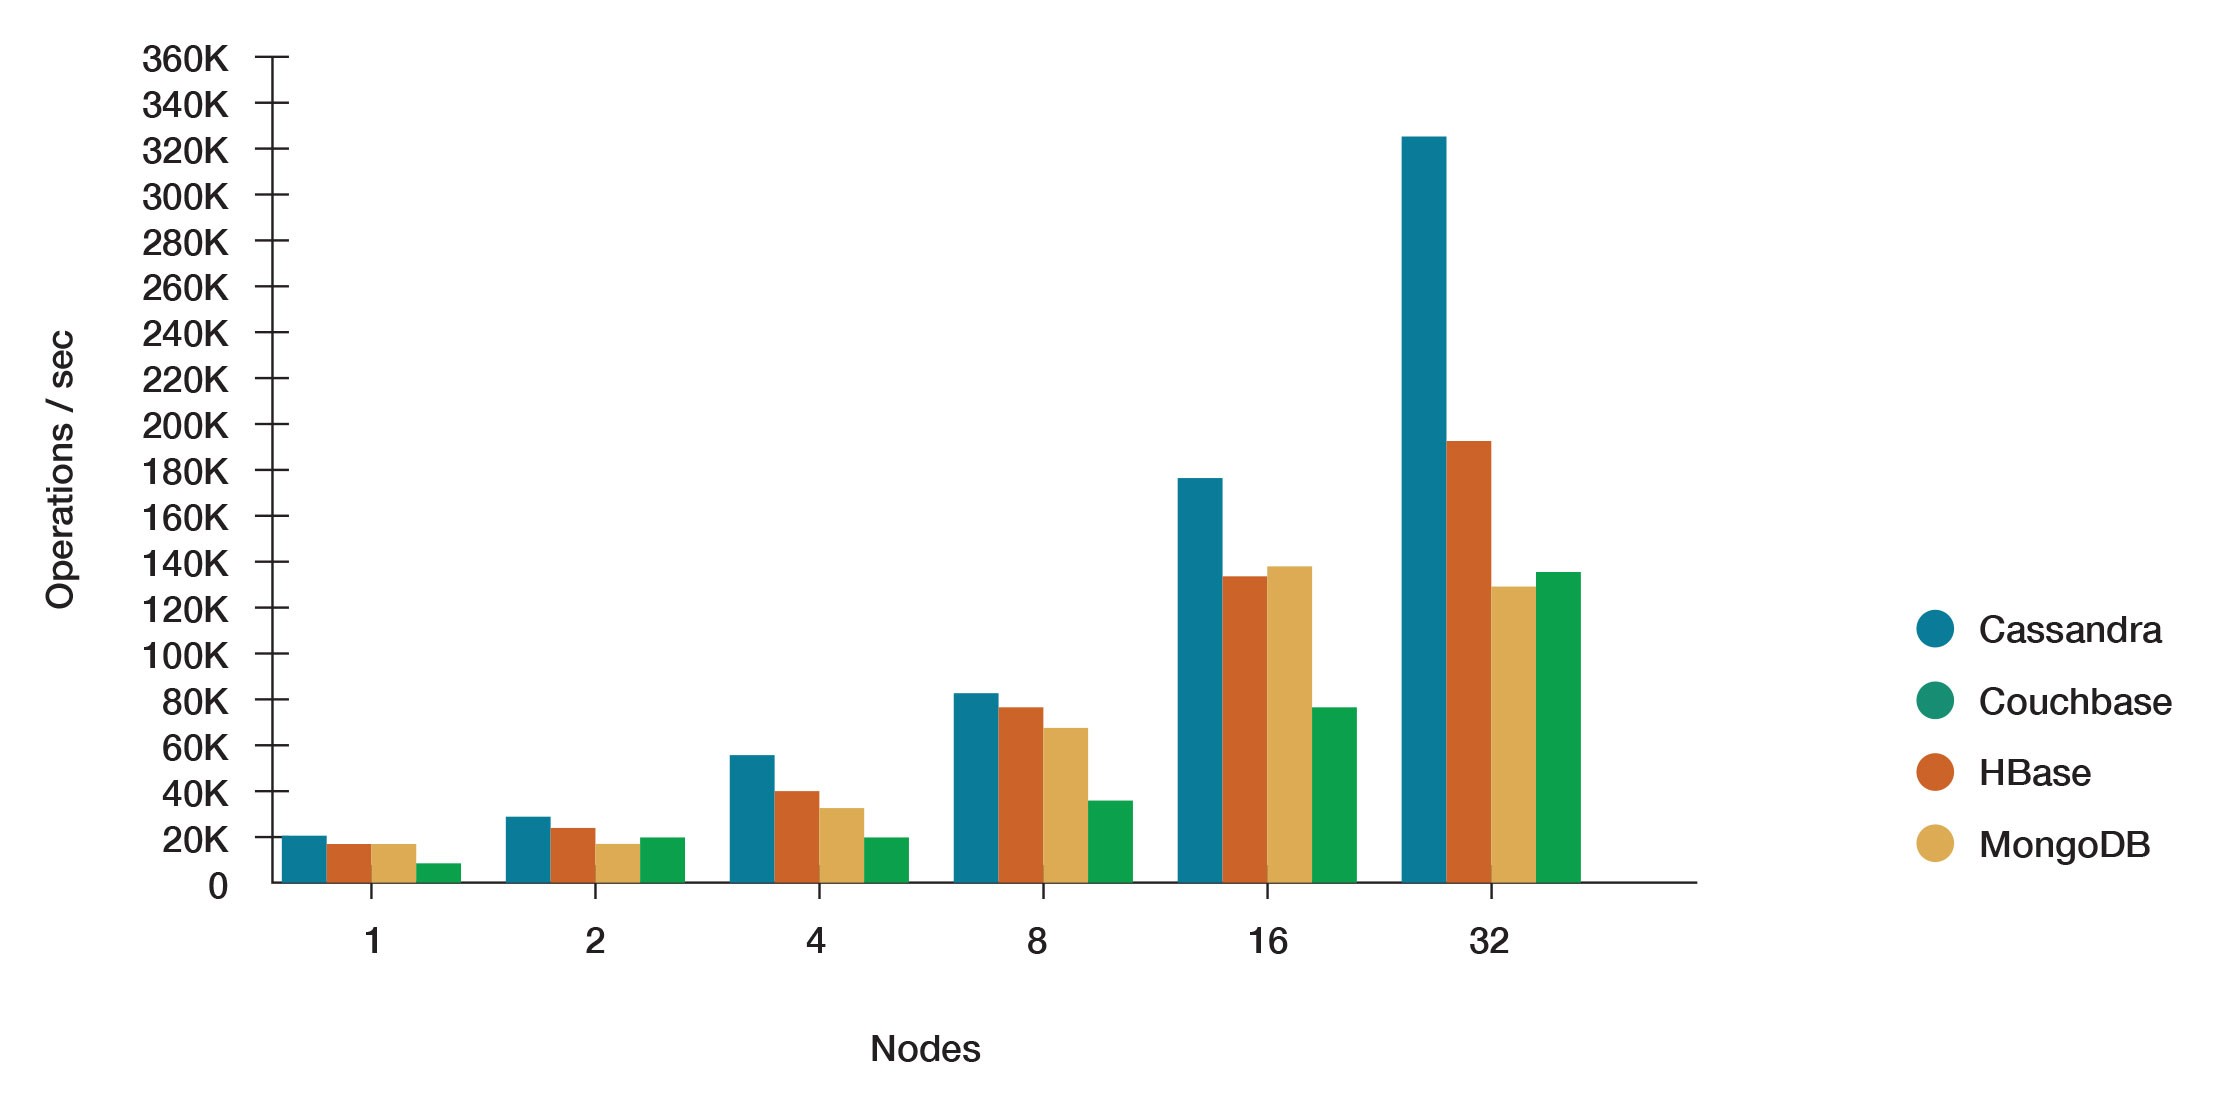
\includegraphics[scale=0.08]{img/grafica.jpg}
          \end{figure}

        \end{frame}
        
        \section{Conclusiones}

        \begin{frame}
          \begin{itemize}
          \item No hay una herramienta única.
          \item Pequeños problemas $\Rightarrow$ gran cantidad de datos.
          \item CC algo indispensable.
          \item Herramientas de alto nivel que facilitan nuestro trabajo.
          \item Cassandra parece una muy buena opción.
          \end{itemize}
        \end{frame}

        	
	\section{Bibliografía}
	
	\begin{frame}
		\begin{itemize}
		\item \href{https://www.infoq.com/articles/traffic-data-monitoring-iot-kafka-and-spark-streaming}{Art. ppal.}
                \item \href{http://kafka.apache.org/intro}{Introducción a Kafka}
                \item \href{http://www.libelium.com/resources/top_50_iot_sensor_applications_ranking/}{50 utilidades del IoT}
                \item \href{https://www.quora.com/What-is-the-actual-role-of-ZooKeeper-in-Kafka}{¿Por qué Zookeeper con Kafka?}
                \item \href{http://spark.apache.org/docs/latest/streaming-programming-guide.html}{Introducción a Spark Streaming}
                \item \href{http://www.datastax.com/nosql-databases/benchmarks-cassandra-vs-mongodb-vs-Hbase}{Comparativa BBDD}
                \item \href{https://scalegrid.io/blog/cassandra-vs-mongodb/}{Cassandra vs. MongoDB}
                \item \href{http://cassandra.apache.org/}{Web de Apache Cassandra}
		\end{itemize}
	\end{frame}
	
	\begin{frame}[plain]
		\begin{center}
			\textcolor{orange}{\textbf{¿Preguntas?}}
		\end{center}
	\end{frame}
	
	
\end{document}